\begin{rightcolumn}

\subsubsection*{\gls{rfr}.} 

Es un método de valuación usado para estimar el valor de ciertos activos intangibles. Se basa en la premisa de que el único valor que el comprador del activo recibe es el ahorro por no tener que pagar regalías a un tercero por el uso de dicho activo. \\

La aplicación de este método involucra estimar el valor de mercado justo de un activo intangible cuantificando el valor presente del flujo de pagos de regalías. \\

Pasos a seguir: \teztit{i) Desarrollar proyecciones de ingresos asociadas al activo intangible bajo análisis. ii) Estimar una tasa de regalías para el activo intangible. iii) Multiplicar el ingreso proyectado por la tasa de regalías estimada. iv) Estimar cualquier gasto (mantenimiento, administrativo, regeneración, etc.) que pueda asociarse al activo. v) Calcular el flujo de ahorros en regalías antes de impuestos y el efecto fiscal para determinar la contribución después de impuestos. vi) Desarrollar una tasa de descuento apropiada para el activo intangible. vii) Aplicar una tasa de descuento o capitalización al flujo de ahorros en regalías después de impuestos y sumar el valor presente de los flujos futuros, incluyendo el valor terminal. viii) Sumar beneficio por amortización fiscal para alcanzar al valor final. (\ref{fig:rfr})

\end{rightcolumn}

\begin{leftcolumn}

\begin{figure}[H]
\label{fig:rfr}\caption{Método RFR Valuation}
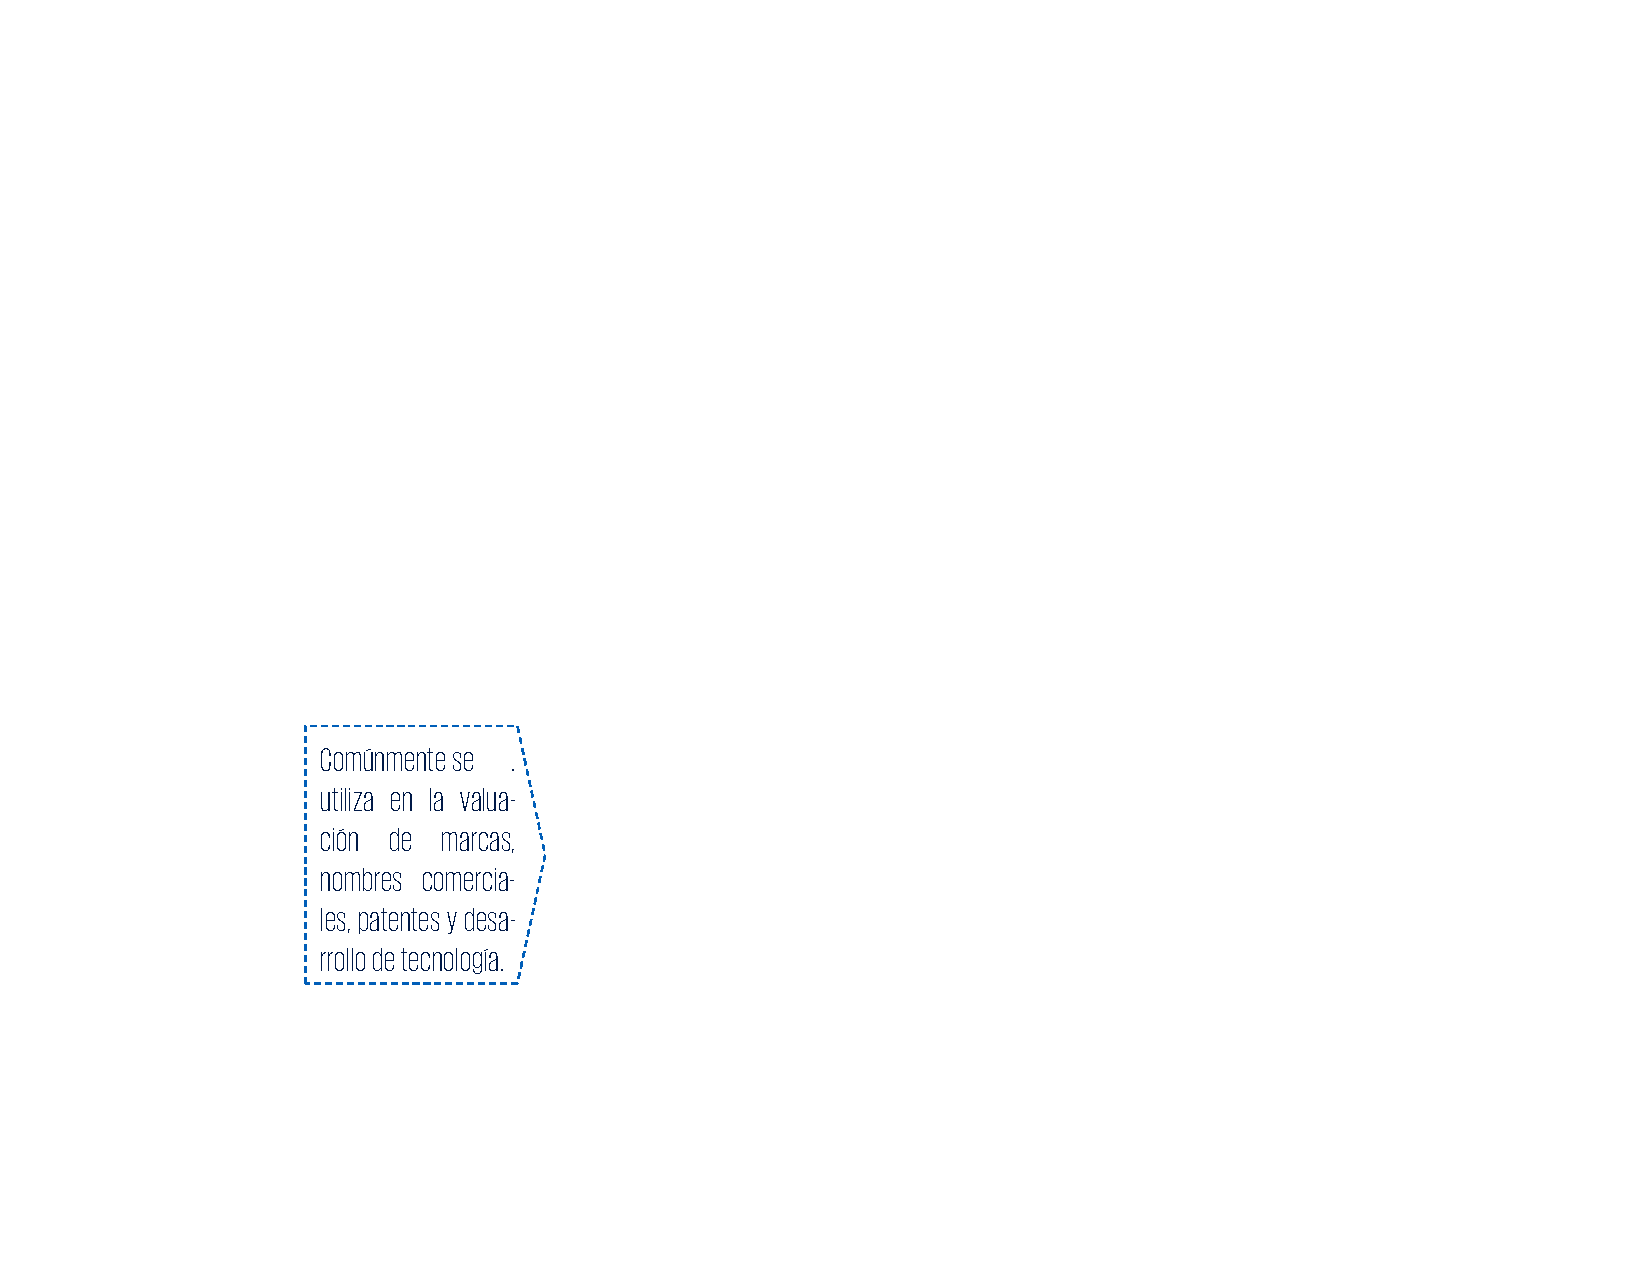
\includegraphics[width=\textwidth]{\rutaImagenes/RFR}\\
\textit{Fuente: KPMG Cárdenas Dosal, S.C. Valuación de Activos Intangibles. Pag. 63. México, 2017.}
\end{figure}

\end{leftcolumn}